% discuss numerical simulation - transfer from L1 to the Moon type orbit
% compare with the transfer using invariant manifolds
\section*{}
\subsection*{Numerical Simulation}
% describe the problem
\begin{frame}%--------------------------------------------%
\frametitle{Transfer Problem}
	\begin{itemize}
		\item Transfer from \( L_1 \) orbit to periodic orbits near the Moon
		\item Bounded control input and fixed time horizon
	\end{itemize}
	\begin{figure}
		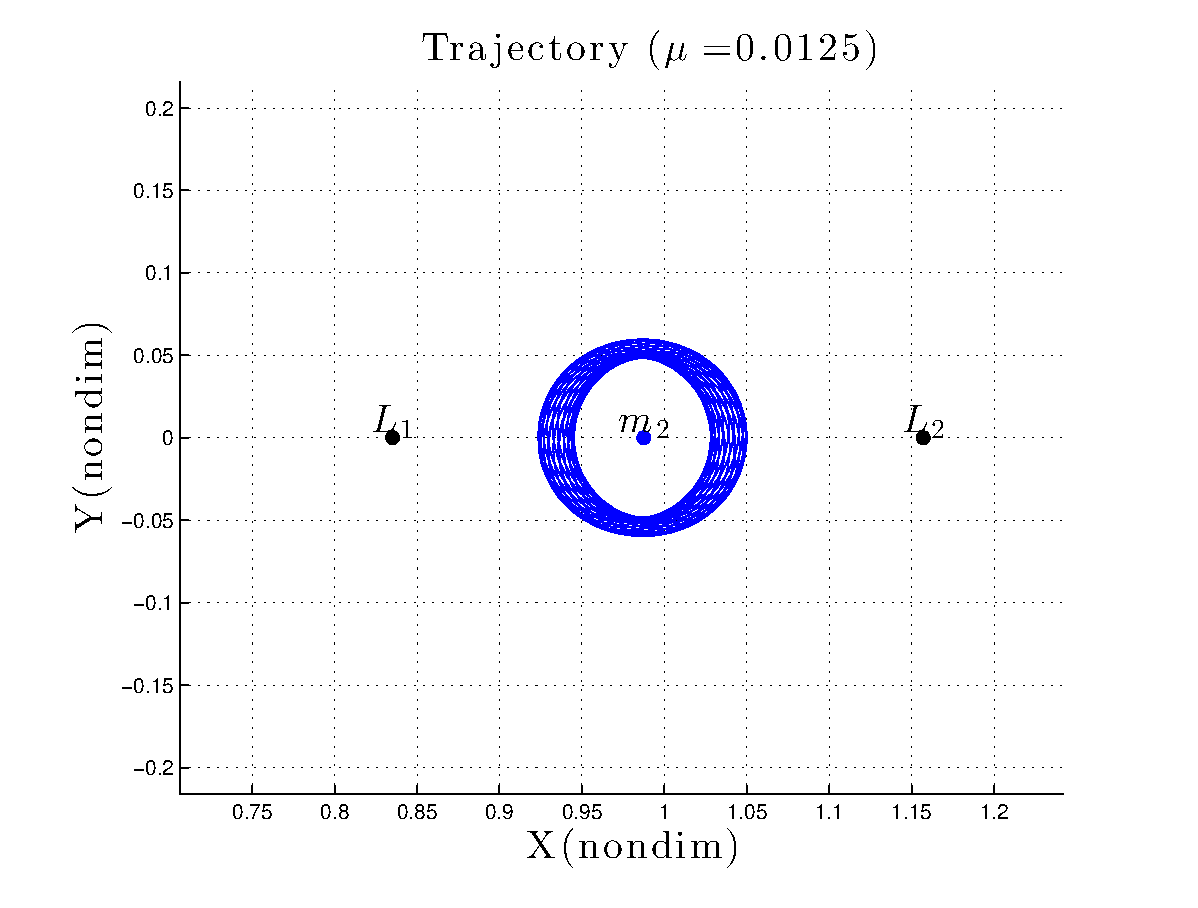
\includegraphics[width=0.7\textwidth]{moon_orbit}
	\end{figure}
	
	\note[itemize]{
		\item Introduce problem
		}
\end{frame} %--------------------------------------------%

% show invariant manifold transfer
\begin{frame} %-----------------------------------------------%
\frametitle{Invariant Manifold Transfer}
\begin{itemize}
	\item Unstable invariant manifolds generated from periodic orbit
	\item Poincar\'e section intersections generated
\end{itemize}
	\begin{figure} 
	\centering 
	\begin{subfigure}[htbp]{0.5\textwidth} 
		\visible<2->{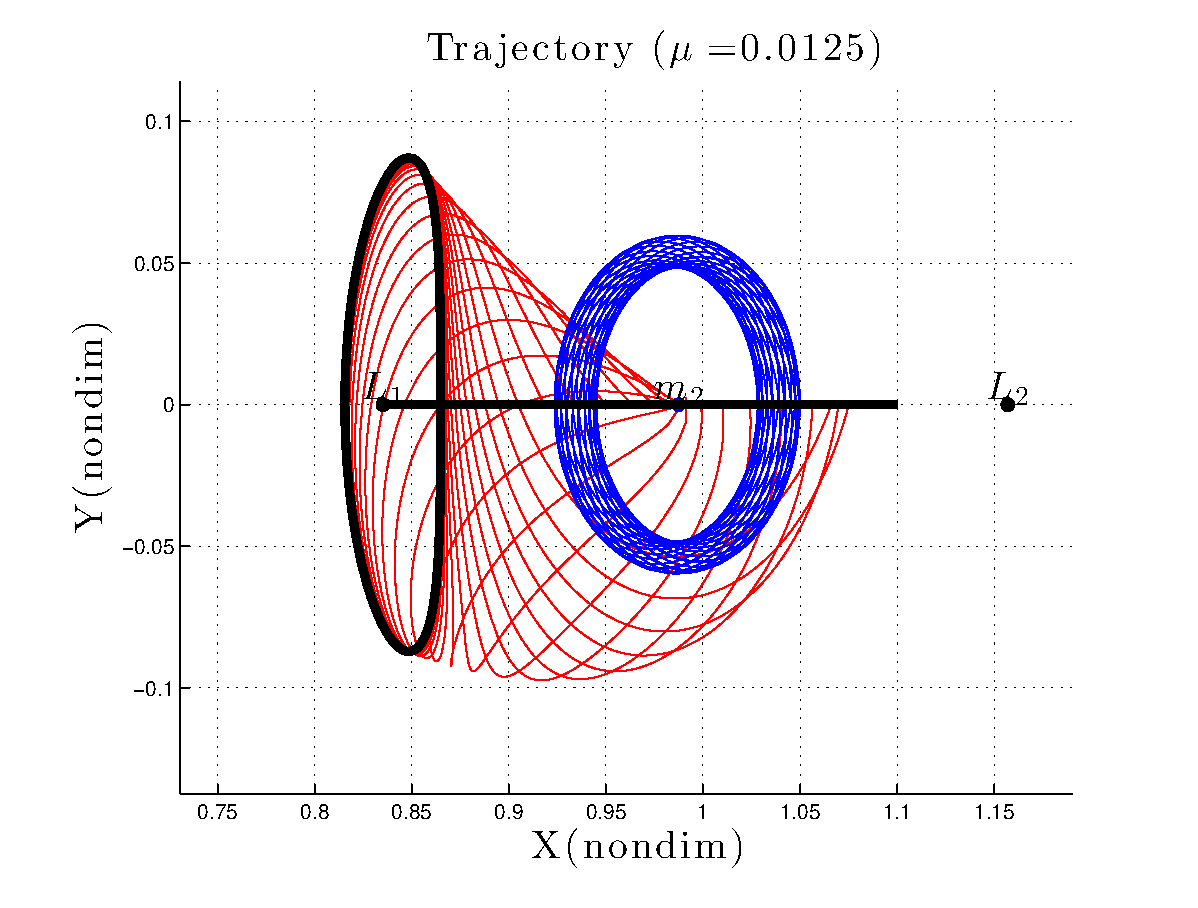
\includegraphics[width=\textwidth]{manifold_trajectory}  }
	\end{subfigure}~
	\begin{subfigure}[htbp]{0.5\textwidth} 
		\visible<3->{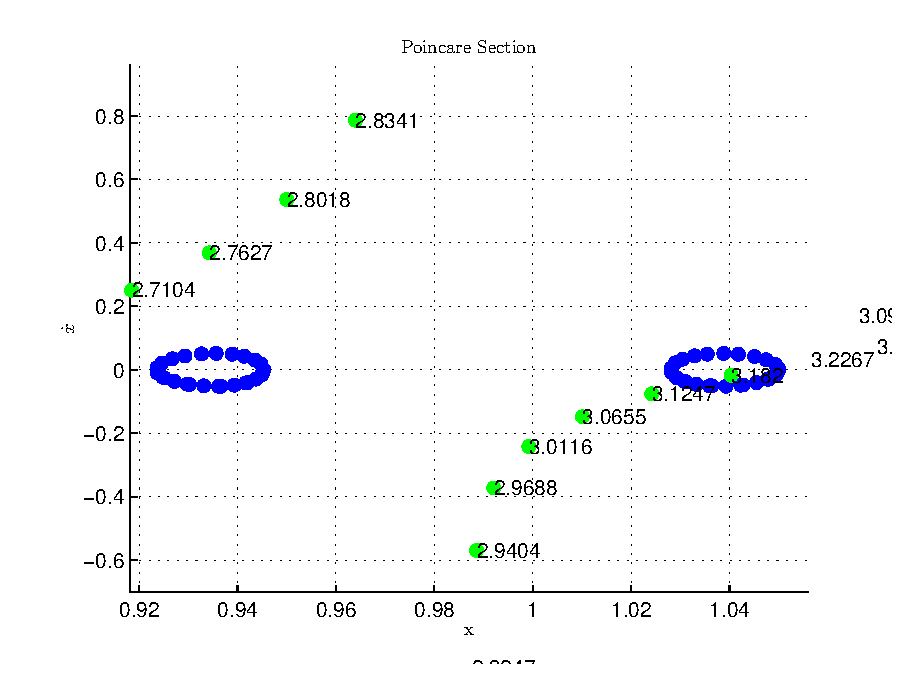
\includegraphics[width=\textwidth]{manifold_poincare} }
	\end{subfigure} 
	\end{figure}
	\visible<4->{
	\begin{itemize}
		\item Only portion of invariant manifold intersects the target
		\item Long time of flight \( t_f \approx 3.1 \)
	\end{itemize}
	}
	\note[itemize]{
		\item Show invariant manifold transfer
		\item Discuss how manifold sometimes don't intersect
		\item Also has a long time of flight
		}
\end{frame} %------------------------------------------------%

% show reachable set transfer
\begin{frame}%------------------------------------------------%
\frametitle{Reachable Set Transfer}
\begin{itemize}
	\item Reachablility set generated on Poincar\'e section
	\item<3-> Intersection point used to generate a transfer
\end{itemize}
	\begin{figure} 
	\centering 
	\begin{subfigure}[htbp]{0.5\textwidth} 
		\only<1-2>{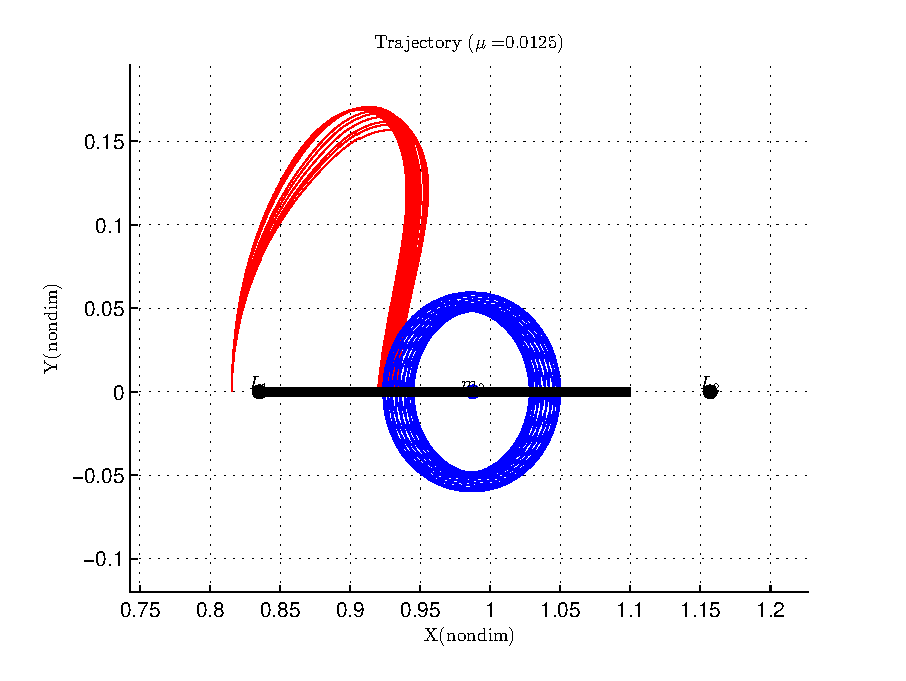
\includegraphics[width=\textwidth]{reach_trajectory}  }
		\visible<3->{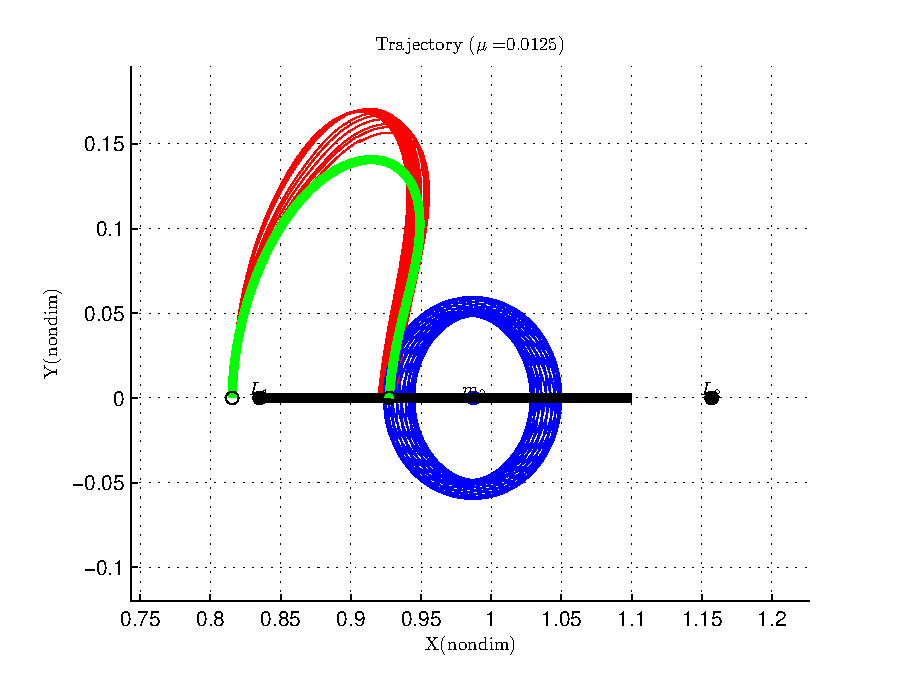
\includegraphics[width=\textwidth]{reach_transfer}  }
	\end{subfigure}~
	\begin{subfigure}[htbp]{0.5\textwidth} 
		\visible<2->{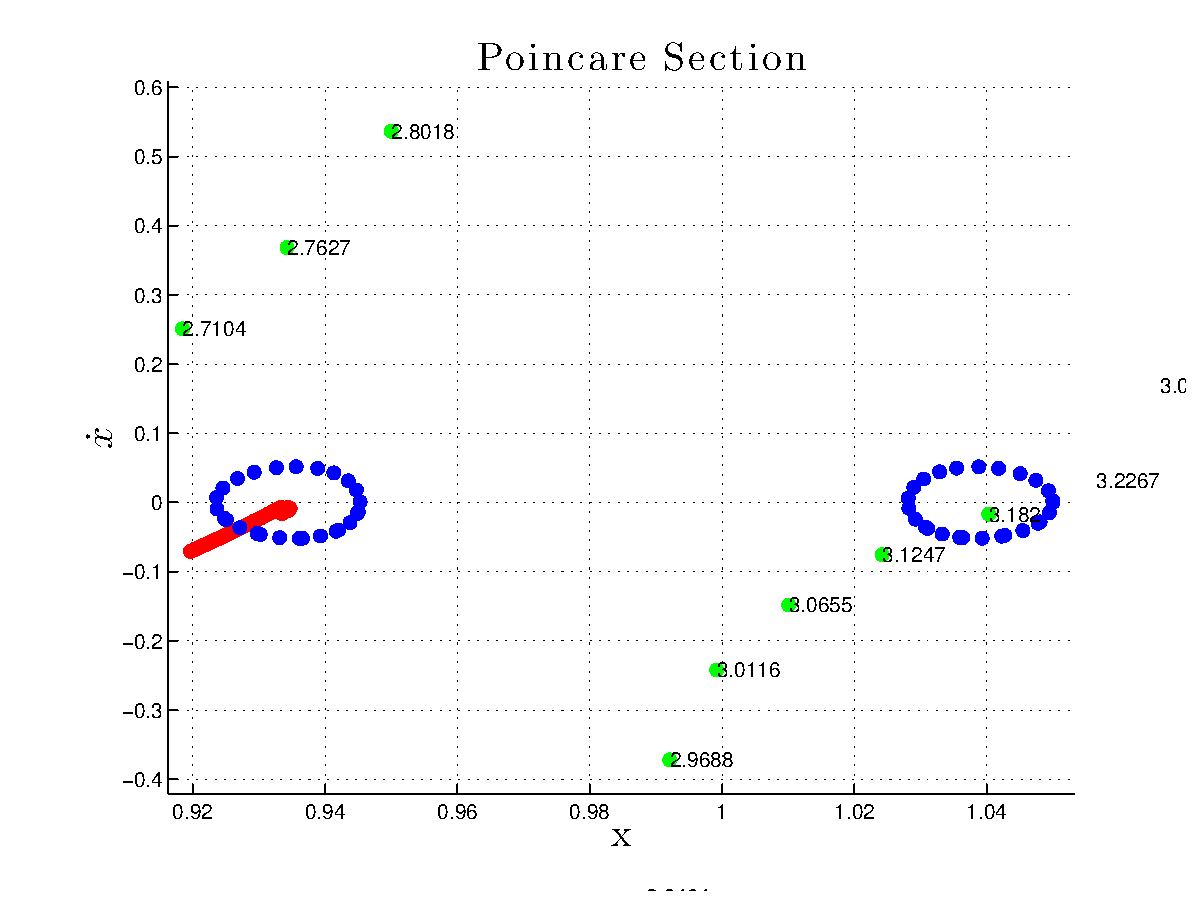
\includegraphics[width=\textwidth]{poincare_compare} }
	\end{subfigure} 
	\end{figure}
	
		\visible<4->{
	\begin{itemize}
		\item  Reachable set intersect the target 
		\item Shorter time of flight \( t_f \approx 1.4 \)
	\end{itemize}
	}
	\note[itemize]{
		\item Compare to reachable set approach
		\item Shorter time of flight
		}
\end{frame} %--------------------------------------------------%